\section{Adding Flow by Data Path Control (dpctl) command}
% \subsection{Overview}
\subsection{Expeimtent Results}

\subsubsection{Simulation scenario python API code}
We set the simulation scenario as followed by the given lecture material:
\vspace{-2mm}
\begin{enumerate}
    \item Setting the 1 host 3 switch topology as the basic topology in Figure 1
    \vspace{-2mm}
    \item After implementing the whole topology then add flow between Host1 h1 and h2 by using 'dpctl' command, then check the pingtest and print out the flow table that doed the host 1 \& host 2 were connected.
\end{enumerate}
The whole scenario implementef by the python scripts below : 
\vspace{-2mm}
\begin{listing}[h!]
\inputminted[framerule = 1pt,framesep = 2mm , frame = lines, fontsize=\scriptsize]{python}{./code/week06/Experiment01.py}
\caption{\footnotesize ex1.py, Experiment 01 simulation scenario python scripts}
\end{listing}
\clearpage
\subsubsection{Terminal out screenshot}
The figure below captures the output of the terminal after executing the Python script code.

By configuring the whole scenario in the python script, it is possible to check the operation of outputting the ping test and flow table before and after adding flow at once.

\begin{figure}[!h]\centering 
	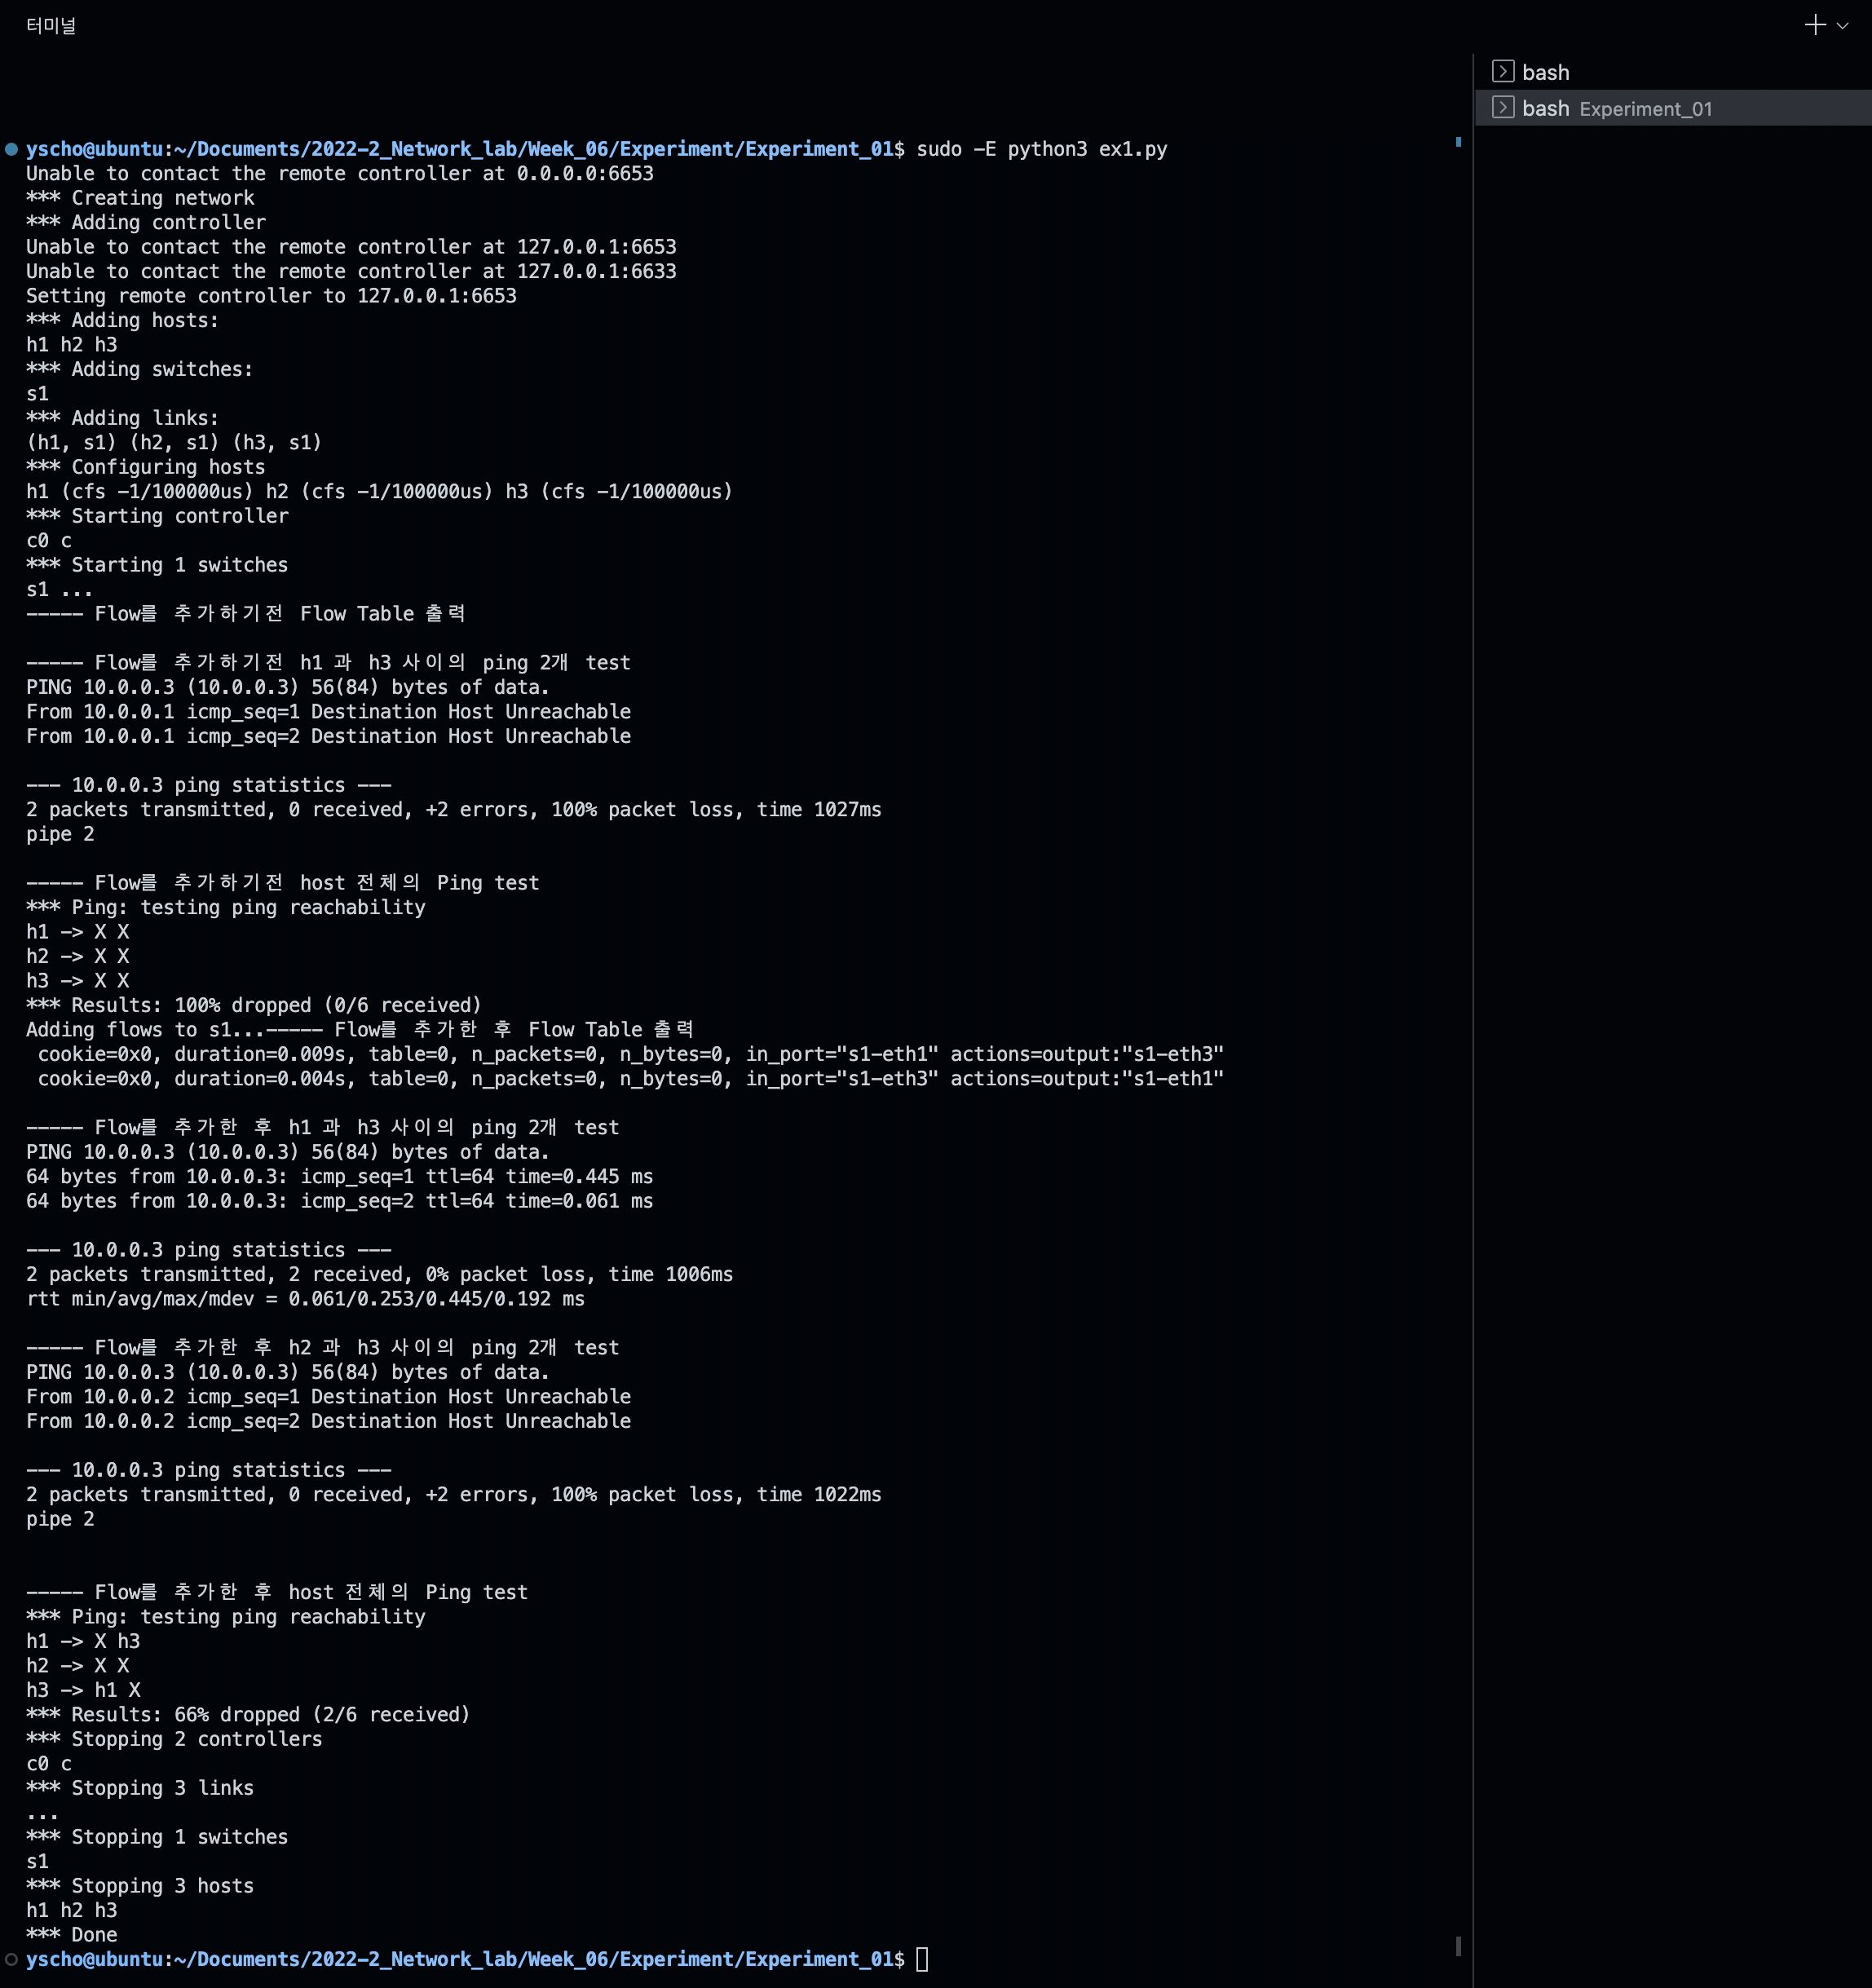
\includegraphics[width=.99\textwidth]{image/week06/1-2.png}
	\caption{
	Terminal out screenshot : Simulation Scenario of Experiment 01}
	\vspace{-10pt}
\end{figure}
\clearpage